\section{Landasan Teori}
\indent

Hasil dari penelitian ini adalah melakukan analisis pergerakan harga saham dan prediksi harga saham di masa yang akan datang dengan menggunakan \textit{Deep Learning}. Deep learning merupakan sebuah konsep kecerdasan buatan yang menggunakan jaringan saraf tiruan untuk memahami serta mempelajari data mulai dari data yang sederhana hingga data yang kompleks. Dengan demikian, proses analisis data saham akan jauh lebih efisien dibandingkan dengan melakukan prosesnya secara manual.

% TODO: ganti referensinya
Algoritma yang akan digunakan untuk melakukan analisis ini adalah \textit{Long Short-Term Memory (LSTM)}. Dengan algoritma ini, memungkinkan model untuk meraih tingkat akurasi yang lebih tinggi dibandingkan dengan model dengan algoritma lain. Dengan akurasi yang lebih tinggi, tentunya akan memudahkan pengguna ataupun investor untuk melakukan analisis dan membantu dalam pengambilan keputusan investasi. Selain itu algoritma LSTM juga dapat mencegah terjadinya permasalahan yang sering terjadi pada saat melakukan proses analisis data saham, yaitu \textit{vanishing gradient} (\cite{sofi2021perbandingan}).

\begin{subs}
	\textbf{\subsection{Saham}}
	% TODO: ganti referensinya
	Investasi merupakan suatu kegiatan penanaman modal berupa uang ataupun harta dengan harapan untuk  mendapatkan keuntungan di masa yang akan datang. Saham merupakan salah satu instrumen investasi yang sangat menarik bagi para investor karena potensi keuntungan yang lebih besar dibandingkan dengan investasi lainnya seperti obligasi dan deposito. Namun perlu diperhatikan bahwa sesuatu yang memiliki keuntungan lebih besar tentunya memiliki risiko yang lebih tinggi juga. Saham seringkali mengalami fluktuasi harga yang membuat saham merupakan investasi dengan risiko yang tinggi. Fluktuasi biasanya dipengaruhi oleh beberapa faktor seperti, kondisi ekonomi internal perusahaan ataupun eksternal, sentimen pasar, serta peristiwa politik maupun sosial lainnya (\cite{Rosyd2024PENERAPANML}).

	\begin{figure}[H]
		\centering
		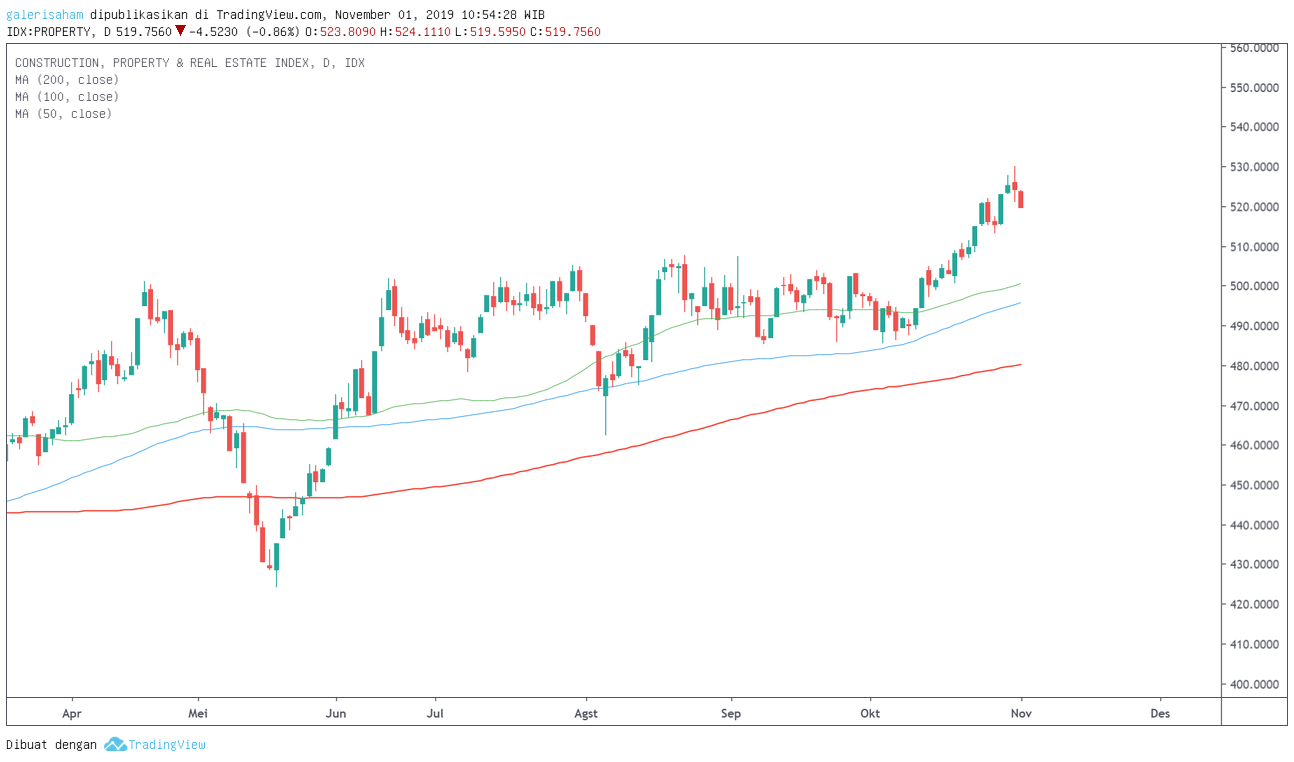
\includegraphics[width=0.8\textwidth]{chart_saham.png}
		\caption{Fluktuasi Harga Saham}
	\end{figure}

	Saham atau pasar modal merupakan sebuah sertifikat/surat yang berharga yang menunjukkan kepemilikan atas suatu perusahaan, dalam sertifikat tercantum nilai saham yang dimiliki, jenis saham yang dimiliki, hak dan kewajiban setiap pemegang saham (\cite{ChristianANALISIS}). Jadi saham merupakan sebuah surat berharga yang menandakan kepemilikan atas suatu perusahaan. Sebagai pemegang saham investor memiliki hak untuk memperoleh hak untuk menerima dividen, hak suara dalam rapat umum pemegang saham dan juga keuntungan dari kenaikan harga saham (\cite{MerissaKeuntunganSaham}).

	Tujuan utama dari investasi saham adalah untuk menghasilkan keuntungan di masa yang akan datang. Artinya investor membeli saham dengan harapan harga saham akan meningkat di masa yang akan datang (\textit{Capital Gain}) yang tentunya menguntungkan investor. Selain dari itu, investasi saham juga dapat memberikan pendapatan pasif (\textit{Pasive Income}) kepada investor yang berupa dividen. Keuntungan dari saham terbagi menjadi dua yaitu, pendapatan dividen dan pertumbuhan saham (\textit{Capital Gain}). Dividen merupakan keuntungan bersih dari perusahaan yang akan dibagikan kepada para pemegang sahamnya. Namun, tidak semua perusahaan membagikan dividen kepada para investor.

	Dengan keuntungan yang tinggi tentunya memilih saham memerlukan beberapa teknik analisis, yaitu analisis fundamental dan juga analisis teknikal. Analisis fundamental merupakan sebuah teknik analisa yang memperhitungkan faktor fundamental sebuah perusahaan yang dapat memengaruhi pergerakan harga saham. Faktor-faktor fundamental ini meliputi, kondisi ekonomi perusahaan, dalam negeri maupun luar negeri, tren pasar/tren industri juga termasuk kedalam faktor fundamental, tingkat persaingan perusahaan, dan juga kebijakan fiskal dan moneter serta yang paling utama yaitu faktor kinerja dari perusahaan yang dapat dicek melalui catatan/laporan keuangan perusahaan tersebut. Selain itu analisis teknikal juga memainkan peran penting dalam memilih saham. analisis teknikal merupakan teknik analisis dengan menggunakan data historis terkait saham seperti menganalisa pergerakan harga saham masa lalu untuk memprediksi harga saham yang akan terjadi di masa depan.
\end{subs}

\begin{subs}
	\textbf{\subsection{Saham LQ45}}
	Indeks LQ45 adalah salah satu indeks saham di Bursa Efek Indonesia (BEI) yang terdiri dari 45 saham yang dipilih berdasarkan kriteria likuiditas dan kapitalisasi pasar yang tinggi. Indeks ini mencakup saham-saham dari perusahaan-perusahaan terkemuka di Indonesia yang dianggap memiliki stabilitas dan daya saing tinggi, serta memainkan peran penting dalam perekonomian Indonesia. Saham-saham dalam LQ45 merupakan representasi dari perusahaan dengan kinerja terbaik dan sering kali menjadi acuan bagi para investor domestik maupun internasional. Saham-saham yang terdaftar dalam LQ45 mencakup berbagai sektor industri seperti perbankan, energi, infrastruktur, dan konsumsi, yang menunjukkan keberagaman sektor yang ada di Indonesia (\cite{kusuma2020saham}).

	Salah satu karakteristik utama dari saham LQ45 adalah likuiditasnya yang tinggi. Saham dengan likuiditas tinggi lebih mudah diperdagangkan karena memiliki volume transaksi yang besar, yang memberikan keuntungan bagi investor dalam hal kemudahan transaksi serta potensi pergerakan harga yang lebih terprediksi. Selain itu, saham-saham dalam LQ45 sering menjadi pilihan utama bagi investor institusional dan fund manager karena saham-saham tersebut dianggap lebih stabil dan cenderung memiliki risiko lebih rendah dibandingkan dengan saham-saham lain di pasar saham Indonesia (\cite{wibowo2018analisis}).

	Pergerakan harga saham dalam LQ45 dapat digunakan untuk menggambarkan kondisi pasar saham Indonesia secara keseluruhan. Oleh karena itu, saham-saham dalam indeks ini sering dianalisis menggunakan berbagai pendekatan, baik itu analisis teknikal maupun analisis fundamental. Dalam analisis teknikal, investor menggunakan berbagai indikator seperti Moving Average (MA), Relative Strength Index (RSI), dan Bollinger Bands untuk mengidentifikasi tren pasar dan memprediksi pergerakan harga saham di masa depan. Sementara itu, dalam analisis fundamental, faktor-faktor yang dianalisis meliputi laporan keuangan perusahaan, manajemen perusahaan, serta faktor makroekonomi yang dapat mempengaruhi kinerja perusahaan-perusahaan yang terdaftar dalam LQ45 (\cite{hutagalung2019analisis}).

	Selain itu, dengan semakin berkembangnya teknologi, terutama dalam bidang kecerdasan buatan, penelitian terkait analisis saham LQ45 mulai mengarah pada penggunaan algoritma machine learning, termasuk deep learning. Salah satu algoritma yang banyak digunakan dalam penelitian ini adalah Long Short-Term Memory (LSTM). LSTM memiliki kemampuan untuk menangani data deret waktu (time series) yang bersifat dinamis dan non-linear, seperti halnya pergerakan harga saham yang sering mengalami fluktuasi. Beberapa penelitian menunjukkan bahwa LSTM lebih efektif dibandingkan dengan model-model lain, seperti Recurrent Neural Networks (RNN), dalam memprediksi pergerakan harga saham (\cite{chairurrachman2022penerapan}; \cite{alim2023pemodelan}). Keunggulan LSTM terletak pada kemampuannya untuk mengatasi masalah vanishing gradient, sehingga lebih efisien dalam melakukan prediksi harga saham berdasarkan data historis.

  Dengan meningkatnya ketertarikan investor untuk menggunakan teknologi dalam analisis pasar saham, LQ45 menjadi salah satu indeks yang sering dianalisis menggunakan metode-metode canggih seperti LSTM. Ini memberikan peluang bagi investor untuk memperoleh informasi yang lebih akurat dan terpercaya, yang pada gilirannya dapat membantu mereka dalam membuat keputusan investasi yang lebih baik dan menguntungkan (\cite{pipin2023deep}).
\end{subs}


\begin{subs}
	\textbf{\subsection{Kecerdasan Buatan}}
	Kecerdasan buatan atau yang lebih biasa dikenal sebagai \textit{Artificial Intelligence} (AI) merupakan teknik yang memungkinkan komputer untuk memahami dan memproses data. \textit{Artificial Intelligence} (AI) merupakan teknik komputer yang memiliki kemampuan untuk menganalisis data dan menemukan solusi untuk masalah yang ada. \textit{Artificial Intelligence} merupakan teknik komputer yang dapat mengambil keputusan dari data yang dikumpulkan. \textit{Artificial Intelligence} memiliki kemampuan untuk menganalisis data, menemukan solusi dan menghasilkan hasil yang relevan (\cite{suleimenov2020artificial}).
	\begin{figure}[H]
		\centering
		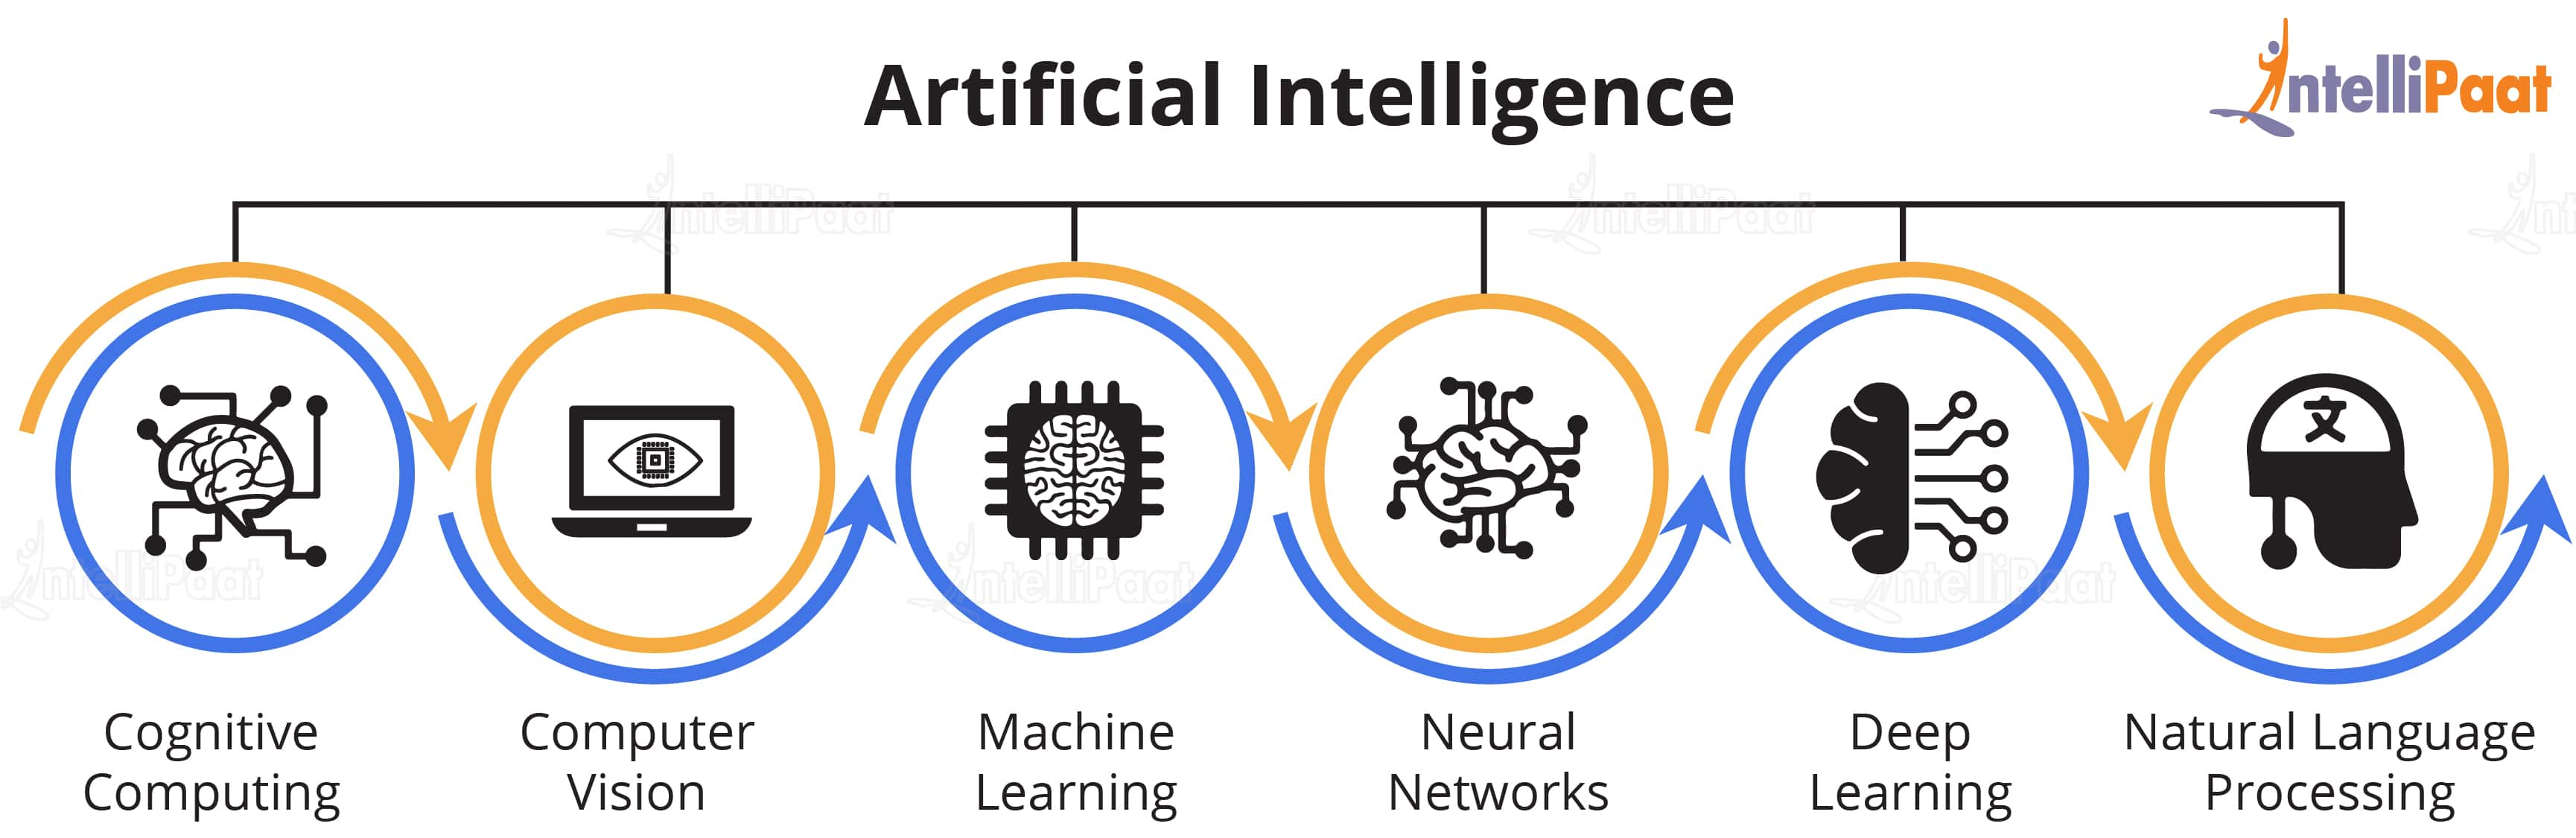
\includegraphics[width=0.8\textwidth]{artificial intelligence.jpg}
		\caption{Pendekatan Kecerdasan Buatan}
	\end{figure}
	Kecerdasan buatan dibuat untuk berfokus untuk melakukan pekerjaan yang biasanya membutuhkan kecerdasan dari manusia. Dengan itu Kecerdasan buatan dibuat guna untuk mempermudah manusia dalam menyelesaikan tugas-tugas/pekerjaan sehari-hari. Ada beberapa pendekatan dalam kecerdasan buatan yaitu,
	% TODO: benerin lagi 20
	\begin{itemize}
		\item Cognitive Computing (Komputasi Kognitif) \\
		      Komputasi kognitif adalah teknologi yang bertujuan untuk meniru cara otak manusia bekerja. Teknologi ini menggabungkan berbagai teknik seperti pembelajaran mesin, pemrosesan bahasa alami, dan analisis data untuk menciptakan sistem yang dapat memahami, bernalar, belajar, dan berinteraksi dengan manusia secara alami. Contohnya adalah IBM Watson, yang mampu menganalisis data dan memberikan wawasan seperti manusia.
		\item Computer Vision (Pengenalan Gambar) \\
		      Computer vision adalah cabang kecerdasan buatan yang berfokus pada bagaimana komputer dapat memahami dan menafsirkan dunia visual, seperti gambar dan video. Teknologi ini digunakan dalam berbagai aplikasi seperti pengenalan wajah, deteksi objek, dan analisis video. Algoritma dalam computer vision memproses gambar dengan cara yang mirip manusia mengenali pola visual.
		\item Machine Learning (Pembelajaran Mesin) \\
		      Machine learning adalah teknik yang memungkinkan sistem komputer belajar dari data tanpa pemrograman eksplisit. Dalam metode ini, algoritma dilatih menggunakan dataset untuk mengenali pola, membuat prediksi, atau mengambil keputusan. Contohnya termasuk rekomendasi produk di e-commerce atau deteksi email spam. Teknologi ini dianggap dasar dalam kecerdasan buatan modern.
		\item Neural Network (Jaringan Saraf Tiruan ) \\
		      Neural network adalah model komputasi yang terinspirasi oleh cara kerja otak manusia, terdiri dari neuron buatan yang terhubung satu sama lain dalam lapisan. Jaringan ini digunakan untuk memproses data kompleks, seperti mengenali pola dalam gambar atau memahami bahasa alami. Contoh penerapannya adalah dalam sistem pengenalan suara dan pemrosesan gambar.
		\item Deep Learning (Pembelajaran Mendalam ) \\
		      Deep learning adalah cabang dari machine learning yang menggunakan jaringan saraf tiruan dengan banyak lapisan (deep neural networks). Teknologi ini dirancang untuk menganalisis data besar dan kompleks, seperti gambar, teks, atau suara, dan menghasilkan prediksi atau keputusan yang lebih akurat. Contoh penerapan deep learning adalah dalam mobil otonom untuk mengenali lingkungan sekitarnya.
		\item Natural Language Processing (Pengenalan Bahasa Alami ) \\
		      Natural Language Processing (NLP) adalah teknologi yang memungkinkan komputer memahami, menganalisis, dan menghasilkan bahasa manusia. Aplikasi dari NLP meliputi asisten virtual seperti Siri atau Alexa, penerjemahan mesin, dan chatbot. Teknologi ini membantu komputer berinteraksi dengan manusia dalam bahasa alami yang digunakan sehari-hari.
	\end{itemize}
\end{subs}

% TODO: masih belum sempurna karena kesempurnaan hanya milik tuhan
% TODO: ganti referensinya
\begin{subs}
	\textbf{\subsection{Python}}
	\begin{figure}[H]
		\centering
		
\includegraphics[width=0.4\textwidth]{python.jpg}
		\caption{Python}
	\end{figure}
	Python merupakan bahasa pemrograman modern dan juga populer yang sering digunakan untuk melakukan pengembangan kecerdasan buatan, termasuk LSTM yang merupakan sebuah model \textit{deep learning}. Python memiliki fitur yang memungkinkan pengguna untuk membuat \textit{script} yang dapat dijalankan secara otomatis. Python merupakan bahasa pemrograman high level yang dimana \textit{syntax}-nya mendekati bahsasa manusia. Python juga memiliki fitur yang memungkinkan pengguna untuk membuat \textit{library} yang dapat digunakan oleh \textit{script} lain untuk mempermudah proses pembuatan aplikasi. Selain itu Python juga memiliki fitur yang memungkinkan pengguna untuk mengakses \textit{package} yang berhubungan dengan \textit{library} tersebut. Dengan demikian, Python dapat digunakan untuk melakukan analisis data saham yang menggunakan LSTM .
	Python memiliki banyak sekali \textit{Library} yang sangat mendukung untuk melakukan pengembangan kecerdasan buatan termasuk LSTM. Dengan demikian, pengguna akan lebih mudah untuk melakukan pembuatan aplikasi kecerdasan buatan yang lebih kompleks. LSTM adalah varian dari jaringan saraf tiruan (Recurrent Neural Networks, RNN) yang dirancang untuk menangani masalah vanishing gradient pada data sekuensial. Model ini sangat cocok untuk tugas-tugas seperti pemrosesan bahasa alami, prediksi deret waktu, dan analisis data sekuensial lainnya (\cite{alim2023pemodelan}).
	Library yang akan digunakan untuk melakukan pemodelan LSTM adalah:
	\begin{itemize}
		\item \textit{NumPy}: \textit{NumPy} adalah sebuah \textit{library} yang digunakan untuk melakukan operasi matematika pada data numerik. Dengan demikian, pengguna dapat melakukan operasi matematika pada data numerik yang berhubungan dengan LSTM.
		\item \textit{Pandas}: \textit{Pandas} adalah sebuah \textit{library} yang digunakan untuk melakukan operasi pada data yang berhubungan dengan LSTM. Dengan demikian, pengguna dapat melakukan operasi pada data yang berhubungan dengan LSTM.
		\item \textit{Matplotlib}: \textit{Matplotlib} adalah sebuah \textit{library} yang digunakan untuk melakukan pembuatan grafik pada LSTM. Dengan demikian, pengguna dapat melakukan pembuatan grafik pada LSTM.
		\item \textit{TensorFlow} \\
		      TensorFlow adalah sebuah pustaka open-source yang digunakan untuk pemodelan jaringan saraf dalam, termasuk Long Short-Term Memory (LSTM). Pustaka ini dikembangkan oleh Google dan mendukung komputasi yang terdistribusi serta pemrograman paralel yang sangat efisien. TensorFlow memungkinkan pengguna untuk membuat dan melatih model LSTM dengan cara yang terstruktur menggunakan API Keras yang lebih tinggi. Dengan dukungan GPU, TensorFlow memungkinkan pelatihan model yang besar dan kompleks dengan lebih cepat. Contoh pemodelan LSTM di TensorFlow meliputi analisis deret waktu, prediksi harga saham, dan banyak aplikasi lain dalam pembelajaran mesin.
		\item \textit{Keras} \\
		      Keras adalah API tingkat tinggi yang dirancang untuk mempermudah pembuatan dan pelatihan model pembelajaran mendalam, termasuk LSTM. Keras pada awalnya berdiri sendiri, namun kini menjadi bagian dari TensorFlow, memanfaatkan kemudahan penggunaan dan fleksibilitas TensorFlow. Keras memudahkan pembuatan arsitektur model LSTM dengan beberapa baris kode yang sederhana. Pengguna cukup mendefinisikan jumlah unit LSTM, memilih optimizer, serta menentukan fungsi aktivasi dan kehilangan (loss function). Keras juga dapat digunakan dengan TensorFlow sebagai backend untuk komputasi, memungkinkan integrasi yang lebih mudah dengan pustaka lain seperti Pandas dan NumPy untuk pra-pemrosesan data.
		\item \textit{scikit-learn (sklearn)} \\
		      scikit-learn adalah pustaka Python yang berfokus pada pembelajaran mesin (machine learning) dan analisis data, yang umumnya digunakan untuk model-model berbasis algoritma yang lebih sederhana seperti regresi, klasifikasi, dan clustering. Meskipun tidak langsung mendukung pemodelan LSTM, scikit-learn sering digunakan bersama dengan pustaka lain (seperti TensorFlow atau Keras) untuk pra-pemrosesan data, seperti normalisasi, pembagian data pelatihan dan pengujian, serta validasi silang. Pustaka ini sangat berguna dalam persiapan data sebelum digunakan untuk pelatihan model pembelajaran mendalam yang lebih kompleks seperti LSTM.
	\end{itemize}
\end{subs}

\begin{subs}
	\textbf{\subsection{Long Short-Term Memory (LSTM)}}
	LSTM merupakan algoritma yang biasa digunakan untuk memproses data time-series. LSTM juga mampu untuk memproses data masa lampau untuk memprediksi data yang akan data/data masa depan. Algoritma ini sering digunakan dikarenakan tingkat akurasi yang tinggi dan kemampuan untuk menganalisis data yang bervariasi/beragam. Selain tingkat akurasi yang tinggi, LSTM juga mampu untuk  mencegah terjadinya permasalahan yang sering terjadi pada saat melakukan proses analisis data yaitu, \textit{vanishing gradient} (\cite{moghar2020stock}).

	% TODO: add references
	Vanishing gradient merupakan salah satu masalah yang seringkali terjadi pada saat melakukan proses pelatihan data pada sebuah jaringan saraf tiruan \textit{(neural network)}. Masalah ini terjadi ketika gradien dari fungsi loss menjadi sangat kecil pada saat \textit{backpropagation} berlangsung. Yang berarti proses pembaruan informasi pada lapisan awal jadi sangat kecil atau tidak lagi berarti/berpengaruh.

	\begin{figure}[H]
		\centering
		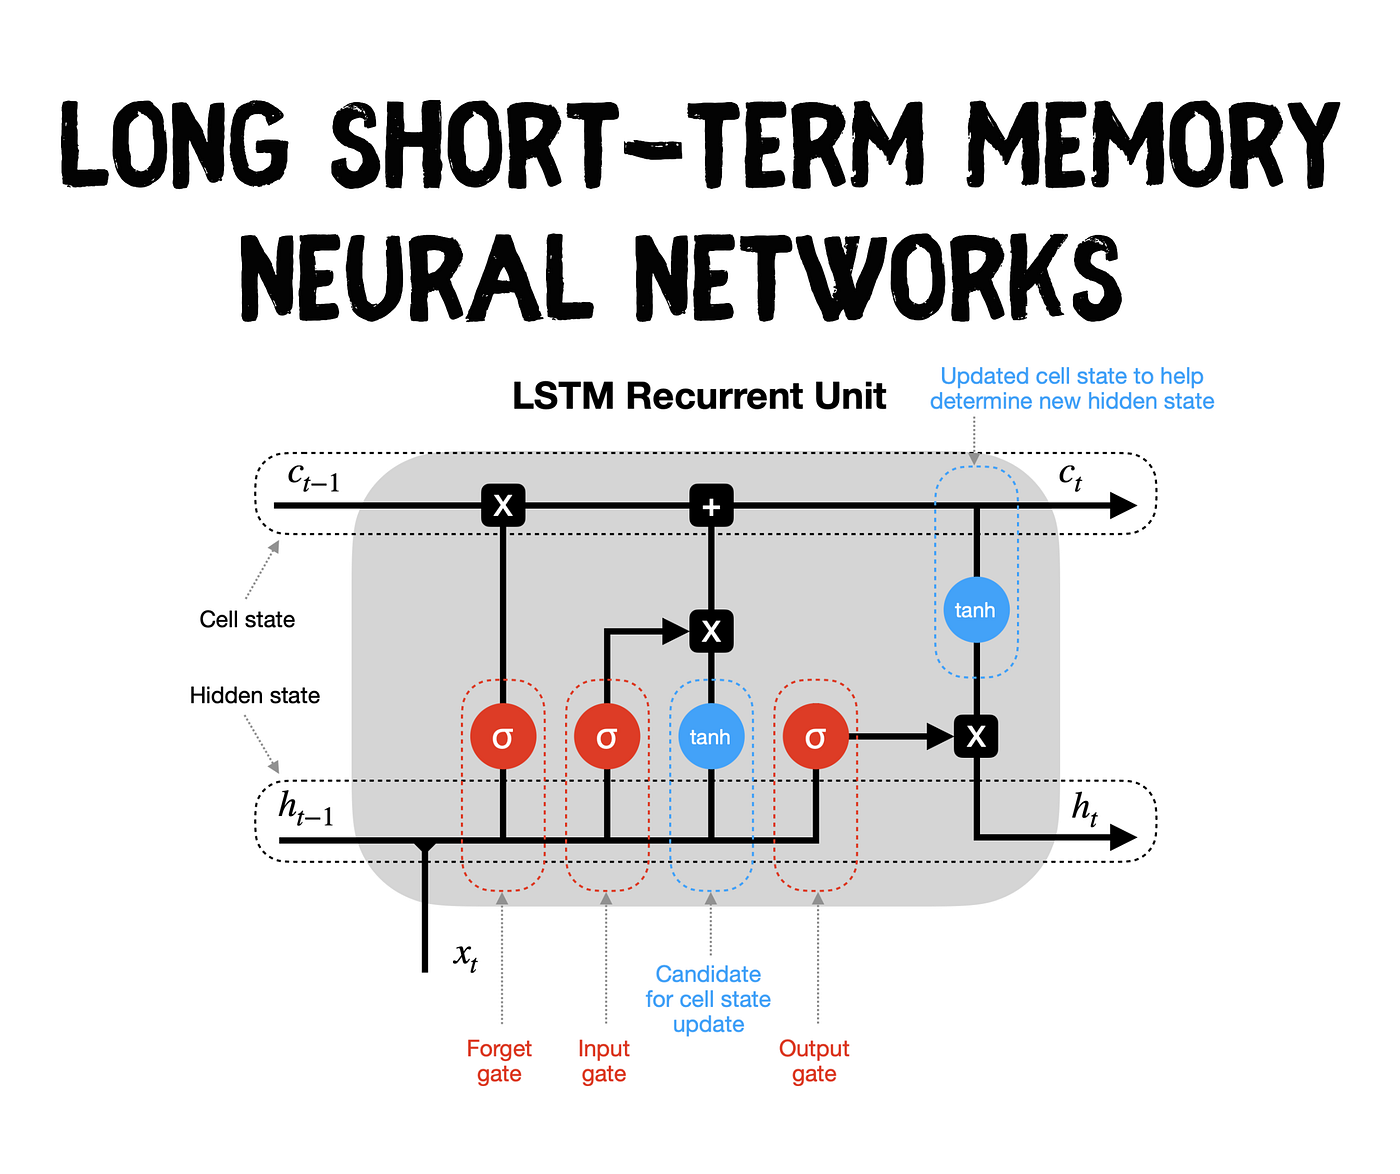
\includegraphics[width=0.8\textwidth]{lstm.png}
		\caption{Algoritma LSTM \textit{(source: \cite{SaulDobilas})}}
	\end{figure}
	LSTM memiliki gerbang \textit{(gate)} yang lebih rumit dibanding algoritma yang lain yang menyebabkan LSTM memiliki tingkat kemampuan akurasi yang jauh lebih tinggi dibanding algoritma lainnya. Namun LSTM memiliki kekurangan yaitu pada tahap \textit{(training)} / proses latihan yang lebih lama. berikut merupakan gerbang-gerbang yang digunakan dalam algoritma LSTM.
	Berikut merupakan langkah-langkah latihan yang dilakukan oleh LSTM:
	\begin{figure}[H]
		\centering
		\begin{subfigure}[b]{0.45\textwidth}
			\centering
			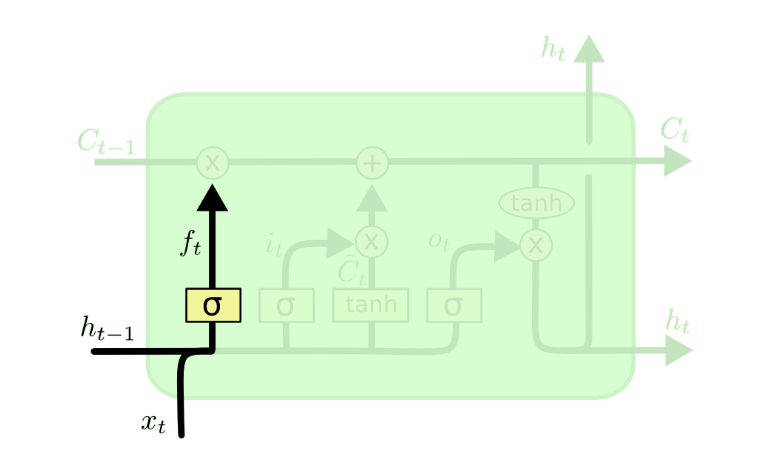
\includegraphics[width=\textwidth]{step1.png}
			% \caption{Forget Gate}
		\end{subfigure}
		\hfill
		\begin{subfigure}[b]{0.5\textwidth}
			\centering
			\[
				f_t = \sigma \left( W_f \cdot \begin{bmatrix} h_{t-1},x_t \end{bmatrix} + b_f \right) ..... (1)
			\]
		\end{subfigure}
		\caption{Forget Gate dengan rumusnya}
	\end{figure}
	Langkah pertama pada proses latihan LSTM adalah menentukan informasi apa yang akan diteruskan ke layer selanjutnya/\textit{cell layer}. Layer ini menggunakan rumus \textit{sigmoid} untuk menentukan hasil antara 0 dengan 1

	\begin{figure}[H]
		\centering
		\begin{subfigure}[b]{0.45\textwidth}
			\centering
			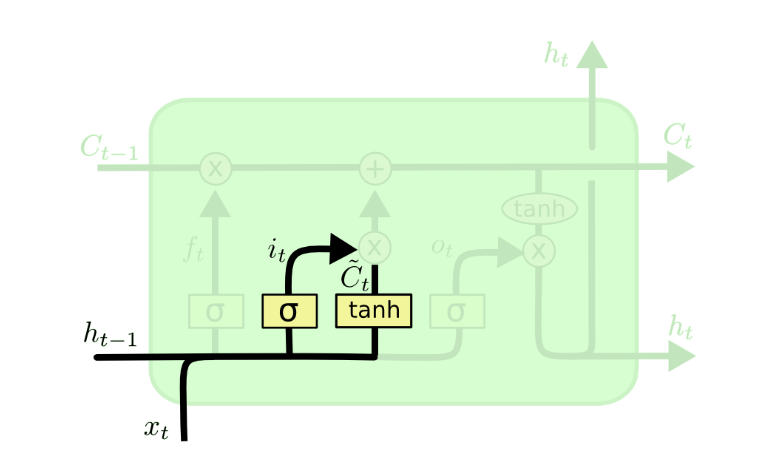
\includegraphics[width=\textwidth]{step2.png} % Replace with your image file
			% \caption{Input Gate}
		\end{subfigure}
		\hfill
		\begin{subfigure}[b]{0.5\textwidth}
			\centering
			\[
				i_t = \sigma \left( W_f \cdot \begin{bmatrix} h_{t-1},x_t \end{bmatrix} + b_i \right)  ..... (2)
			\]
			\[
				C_t = \tanh \left( W_C \cdot \begin{bmatrix} h_{t-1},x_t \end{bmatrix} + b_C \right) ..... (3)
			\]
		\end{subfigure}
		\caption{Input Gate dengan rumusnya}
	\end{figure}
	Selanjutnya adalah proses \textit{Input Gate}, yaitu proses untuk menambahkan informasi baru ke \textit{Cell Layer}. Dalam layer ini juga memutuskan informasi baru apa yang akan disimpan kedalam \textit{Cell State}

	\begin{figure}[H]
		\centering
		\begin{subfigure}[b]{0.45\textwidth}
			\centering
			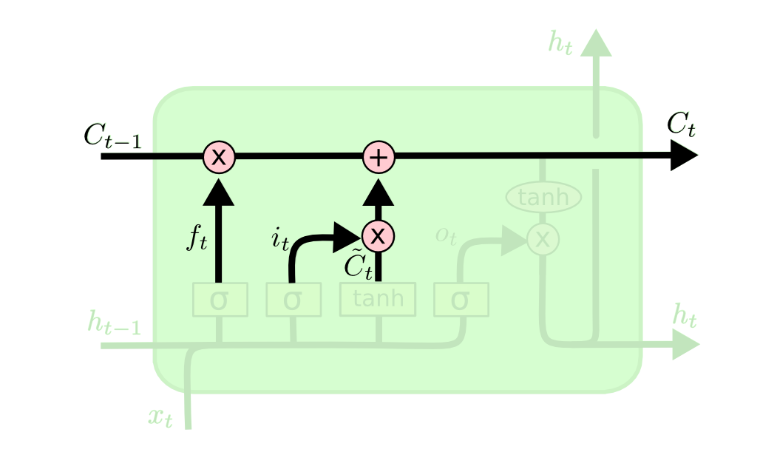
\includegraphics[width=\textwidth]{step3.png}
			% \caption{Pembaruan Cell State}
		\end{subfigure}
		\hfill
		\begin{subfigure}[b]{0.5\textwidth}
			\centering
			\[
				f_t = \sigma \left( W_f \cdot \begin{bmatrix} h_{t-1},x_t \end{bmatrix} + b_f \right) ..... (4)
			\]
		\end{subfigure}
		\caption{Pembaruan Cell State dengan rumusnya}
	\end{figure}
	Selanjutnya adalah proses pembaruan \textit{Cell State}. Informasi yang sudah dipilih dalam layer sebelumnya akan dijadikan data yang baru dan data yang lama akan dihapus. Hal ini memastikan bahwa LSTM akan selalu bekerja dengan informasi yang relevan untuk menghasilkan prediksi yang akurat.

	\begin{figure}[H]
		\centering
		\begin{subfigure}[b]{0.45\textwidth}
			\centering
			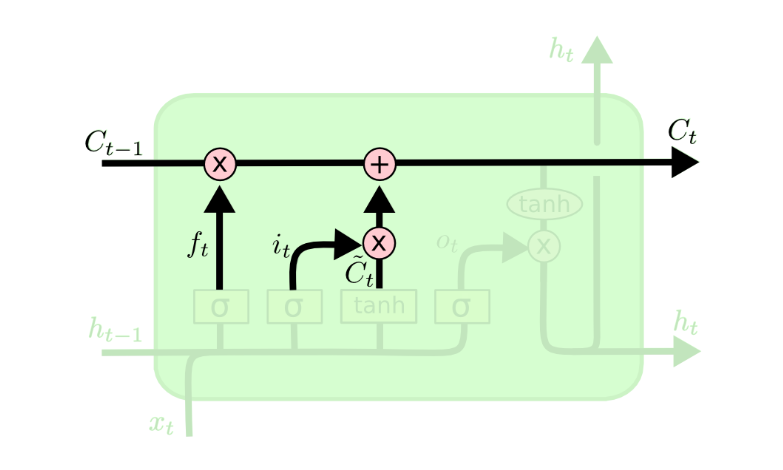
\includegraphics[width=\textwidth]{step4.png}
			% \caption{Output Gate}
		\end{subfigure}
		\hfill
		\begin{subfigure}[b]{0.5\textwidth}
			\centering
			\[
				f_t = \sigma \left( W_f \cdot \begin{bmatrix} h_{t-1},x_t \end{bmatrix} + b_f \right) ..... (5)
			\]
		\end{subfigure}
		\caption{Output Gate dengan rumusnya}
	\end{figure}
	Langkah terakhir adalah proses \textit{Output Gate}, yaitu proses menentukan informasi apa yang akan dihasilkan sebagai output. Proses ini memiliki 3 proses penyaringan sebelum menjadi sebuah output, yaitu Pemfilteran awal dengan sigmoid layer, Normalisasi dengan fungsi tanh dan Kombinasi hasil (\cite{Christopher}).

\end{subs}
